\documentclass{article}
\usepackage[utf8]{inputenc}

\title{Übung 3}
\author{Laurenz Weixlbaumer, 11804751}
\date{November 2018}

\renewcommand{\arraystretch}{1.3}
\renewcommand\thesubsection{(\alph{subsection})}

\usepackage{enumitem}
\usepackage{mathtools}

\begin{document}

\maketitle

\stepcounter{section}\stepcounter{section}
\section{Multiplexer}

\begin{enumerate}[label=(\alph*)]

\item Multiplexer Schaltfunktion

$$
(\overline{sel} \land I_1) \lor (sel \land I_0)
$$

\addtocounter{enumi}{1}

\item Multiplexer Gatterschaltung

\begin{figure}[htp]
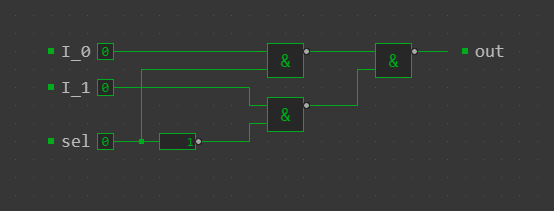
\includegraphics[width=\linewidth]{mux_circuit.png}
\end{figure}

\item In der Schaltung werden 3 NAND-Gatter verwendet, und der längste Weg durchläuft 2 Gatter.

\end{enumerate}

\end{document}
